{\section{Wstęp}}

Gęstość jest to wielkość fizyczna, którą matematycznie opisuje się jako stosunek masy substancji do jej objętości,
a jednostką w układzie SI są kilogramy na metry sześcienne.

$$\rho = \frac{m}{V} \quad [\frac{kg}{m^3}]$$

{\noindent \small gdzie: \\ $\rho$ - gęstość \\ $m$ - masa substancji \\ $V$ - objętość substancji } \\

W przypadku, gdy mamy do czynienia z substancją jednorodną nie będzie miało znaczenia jaki wybierzemy jej "skrawek", ponieważ gęstość będzie przyjmowała tę samą wartość.
W tym eksperymencie posłużymy się jednak całą objędością modeli. \\

Do pomiaru gęstości potrzebujemy zmierzyć dwie wielkości fizyczne: objętość oraz masę.
Do pomiaru objętości stosuje się dwie metody.
Jedną z nich jest pomiar objętości poprzez dokonanie pomiarów obiektu używając suwmiarki,
bądź mikrometru. Metoda ta jest dosyć dokładna,
ponieważ suwmiarka posiada błąd systematyczny o wartości $0.05mm$,
aczkolwiek przy bardziej skomplikowanych detalach ilość pomiarów zwiększa błąd pomiarowy.
Drugą metodą pomiaru objętości jest użycie menzurki z wodą,
która przy pomiarze miała błąd systematyczny o wartości $\pm 1mL$. \\

Pomiary zostały zebrane z dwóch elementów: cylindra (model po lewej), oraz wałka (model po prawej).

\begin{figure}[h]
    \centering
    
\includegraphics[width=70mm]{imgs/rysunek_cylindra.png}
    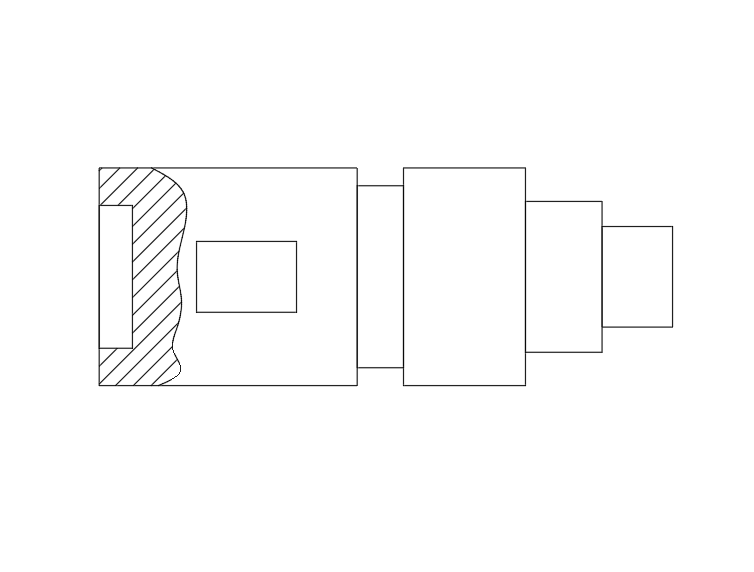
\includegraphics[width=70mm]{imgs/rysunek_walca.png}
    \caption{Uproszczone rysunki techniczne dla obu modeli}
    \label{fig:rysunki}
\end{figure}

\pagebreak

Do wyznaczenia gęstośći, z uwzględnieniem błędów pomiarowych, obu wyżej widocznych modeli użyte zostaną poniższe wzory: \\

Gęstość \hfill $\rho = \frac{m}{V}$ \\

Objętość cylindra \hfill $V_{cyl} = \pi r^2 \cdot h$ \\
{
\indent \qquad \small gdzie $r$ - promień podstawy \\
\indent \qquad \small $h$ - wysokość cylindra \\
}

Niepewność standardowa typu A \hfill $\displaystyle u_A(x) = \sqrt{ \frac{ \displaystyle \sum_{i=1}^{n} (x_i - \overline{x} )^2 }{ n(n - 1) } }$ \\
{
\indent \qquad \small gdzie $x_i$ - kolejny wynik pomiaru \\
\indent \qquad \small $\overline{x}$ - średnia arytmetyczna pomiarów \\
}

Niepewność standardowa typu B \hfill $\displaystyle u_B(x) = \sqrt{ \frac{ (\Delta_p x)^2 }{3} }$ \\
{
\indent \qquad \small gdzie $\Delta_p x$ - bład systematyczny przyrządu pomiarowego \\
}

Niepewność standardowa całkowita \hfill $\displaystyle u(x) = \sqrt{ u_A^2 + u_B^2 }$ \\

Niepewność złożona \hfill $\displaystyle u_c(y) = \sqrt{\displaystyle\sum_{i=1}^{n} \left( \frac{\partial f}{\partial x_i} \right)^2 u^2(x_i)} $ \\
